\section{Resultados}%
\label{sec:resultados}

Nesta seção, são apresentados os resultados obtidos a partir da execução dos experimentos descritos na \autoref{sec:metodologia}.

\subsection{Análise dos Resultados}%

A partir dos resultados obtidos, é possível analisar o desempenho dos algoritmos em cada um dos problemas propostos.
Foi considerado o valor de \gls{fitness} do ótimo global ideal como 263.895843.

Com base nos valores de \gls{fitness} das execuções, foram calculados:

\begin{symbols}
    \item[\( \Delta \)] a discrepância em relação ao ótimo global ideal;
    \item[\( \sigma^{2} \)] a variância dos valores de \gls{fitness} obtidos;
    \item[\( \sigma \)] o desvio padrão dos valores de \gls{fitness} obtidos.
\end{symbols}

O experimento consistiu em executar cada algoritmo 10 vezes, variando os pesos atribuídos às penalizações por violação das restrições. Inicialmente, testaram-se pesos de 100, 200, 400 e 800, com o valor dobrando a cada execução. Posteriormente, o peso foi reduzido gradualmente, sendo testados 50, 25, 12,5 e, por fim, 0.

As tabelas~\ref{tab:resultados-genetico} e~\ref{tab:resultados-memetico} apresentam, para os otimizadores \gls{esga} e \gls{oma}, respectivamente, os resultados obtidos.
Elencam-se os valores de \gls{fitness} e de discrepância da melhor solução e da média das 10 execuções realizadas para cada peso de penalização, além de os valores de variância e desvio padrão entre as soluções encontradas.
Os dados completos do experimento com o algoritmo genético%
\footnote{%
    Resultados do experimento para o algoritmo genético. Disponível em: \url{https://docs.google.com/spreadsheets/d/1589Xh2bLunegQypvfnBg_3csuZElcqJtsFiOOzEYmz8/edit?usp=sharing}.
}
e com o memético%
\footnote{%
    Resultados do experimento para o algoritmo memético. Disponível em: \url{https://docs.google.com/spreadsheets/d/1d157cRAJqgtAQ1KfIHSeW07LFzINioJR8bucLpOU43w/edit?usp=drive_link}.
}
estão disponíveis on-line.

\begin{table}[!ht]
    \resizebox{\textwidth}{!}{%
        \begin{tabular}{lrrrrrrr}
            \bottomrule
            \textbf{Weight}                                &
            \textbf{Best fitness}                          &
            \textbf{Average fitness}                       &
            \textbf{Best \(\boldsymbol{\Delta}\)}          &
            \textbf{Average \(\boldsymbol{\Delta}\)}       &
            \textbf{Fitness \( \boldsymbol{\sigma^{2}} \)} &
            \textbf{Fitness \( \boldsymbol{\sigma}\)}
            \\ \midrule
            0                                              &
            \textbf{0.664898658369470}                     &
            \textbf{1.351379134170120}                     &
            261.310316805323000                            &
            262.544463865830000                            &
            0.436608119613905                              &
            0.660763285612862
            \\
            12.5                                           &
            178.997677252294000                            &
            179.104808940107000                            &
            84.504691568419000                             &
            84.791034059893200                             &
            0.013390962925215                              &
            0.115719328226597
            \\
            25                                             &
            216.367732200399000                            &
            216.393958331948000                            &
            47.428849151152000                             &
            47.501884668051500                             &
            0.000845483185771                              &
            0.029077193567664
            \\
            50                                             &
            263.916813724328000                            &
            263.963887551704000                            &
            0.020970724327981                              &
            0.068044551704293                              &
            0.000929526320056                              &
            0.030488134086159
            \\
            100                                            &
            263.907667139552000                            &
            263.929150603033000                            &
            0.011824139552005                              &
            \textbf{0.033307603033092}                     &
            0.000268368246443                              &
            0.016381948798706
            \\
            200                                            &
            263.897546338518000                            &
            263.940946098212000                            &
            \textbf{0.001703338517984}                     &
            0.045103098212383                              &
            0.000428792341542                              &
            0.020707301648019
            \\
            400                                            &
            263.904722244638000                            &
            263.941341028093000                            &
            0.008879244637967                              &
            0.045498028093277                              &
            0.000678108343263                              &
            0.026040513498460
            \\
            800                                            &
            263.901900217279000                            &
            263.931432135312000                            &
            0.006057217278965                              &
            0.035589135312284                              &
            \textbf{0.000207542501157}                     &
            \textbf{0.014406335452058}
            \\ \toprule
        \end{tabular}%
    }
    \caption{Resultados obtidos para o \gls{problem} em que se varia o peso da função de penalização, tendo sido aplicado o otimizador \gls{esga}.
    }%
    \label{tab:resultados-genetico}
\end{table}
\begin{table}[!ht]
    \resizebox{\textwidth}{!}{%
        \begin{tabular}{lrrrrrrr}
            \bottomrule
            \textbf{Weight}                                &
            \textbf{Best fitness}                          &
            \textbf{Average fitness}                       &
            \textbf{Best \(\boldsymbol{\Delta}\)}          &
            \textbf{Average \(\boldsymbol{\Delta}\)}       &
            \textbf{Fitness \( \boldsymbol{\sigma^{2}} \)} &
            \textbf{Fitness \( \boldsymbol{\sigma}\)}
            \\ \midrule
            0                                              &
            \textbf{0.000000000000000}                     &
            \textbf{0.000000000000000}                     &
            263.895843000000000                            &
            263.895843000000000                            &
            \textbf{0.000000000000000}                     &
            \textbf{0.000000000000000}
            \\
            12.5                                           &
            75.000000000000000                             &
            75.000000000000000                             &
            188.895843000000000                            &
            188.895843000000000                            &
            0.000000000000000                              &
            0.000000000000000
            \\
            25                                             &
            150.000000000000000                            &
            150.000000000000000                            &
            113.895843000000000                            &
            113.895843000000000                            &
            0.000000000000000                              &
            0.000000000000000
            \\
            50                                             &
            266.274169979695000                            &
            266.274169979695000                            &
            2.378326979694980                              &
            2.378326979694980                              &
            0.000000000000000                              &
            0.000000000000000
            \\
            100                                            &
            266.274169979695000                            &
            266.274169979695000                            &
            2.378326979694980                              &
            2.378326979694980                              &
            0.000000000000000                              &
            0.000000000000000
            \\
            200                                            &
            266.274169979695000                            &
            266.274169979695000                            &
            2.378326979694980                              &
            2.378326979694980                              &
            0.000000000000000                              &
            0.000000000000000
            \\
            400                                            &
            265.600129207775000                            &
            266.206765902503000                            &
            \textbf{1.704286207775000}                     &
            \textbf{2.310922902502980}                     &
            0.045433096221042                              &
            0.213150407508505
            \\
            800                                            &
            266.274169979695000                            &
            266.274169979695000                            &
            2.378326979694980                              &
            2.378326979694980                              &
            0.000000000000000                              &
            0.000000000000000
            \\ \toprule
        \end{tabular}%
    }
    \caption{Resultados obtidos para o \gls{problem} em que se varia o peso da função de penalização, tendo sido aplicado o otimizador \gls{oma}.
    }%
    \label{tab:resultados-memetico}
\end{table}

Em todas as execuções com pesos iguais ou superiores a 100, o algoritmo genético simples convergiu para soluções muito próximas do ótimo.
O experimento com peso de 100 apresentou uma convergência total antes de 200 gerações, como mostrado na \autoref{fig:ga-weight-100}.
Com pesos de 400, a convergência foi um pouco mais lenta, ocorrendo pouco após 600 gerações, como mostrado na \autoref{fig:ga-weight-400}.

Mesmo com penalizações elevadas, como 800, a convergência se manteve consistente, tendo encontrado uma solução próxima do ótimo global pouco antes da geração 800, como mostrado na \autoref{fig:ga-weight-800}.
Entretanto, com esses pesos mais altos, o algoritmo exigiu um número maior de iterações para alcançar a solução final, embora a qualidade dessa tenha permanecido satisfatória.

\begin{figure}
    \centering
    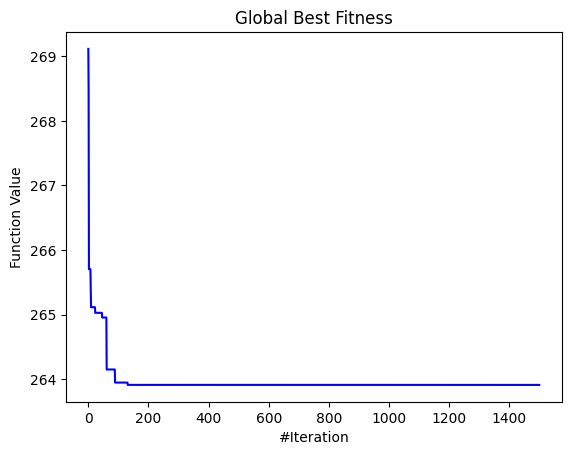
\includegraphics[width=.6\linewidth]{images/weight/100.png}
    \caption{Convergência do algoritmo genético com peso de penalização de 100.}%
    \label{fig:ga-weight-100}
\end{figure}

\begin{figure}
    \centering
    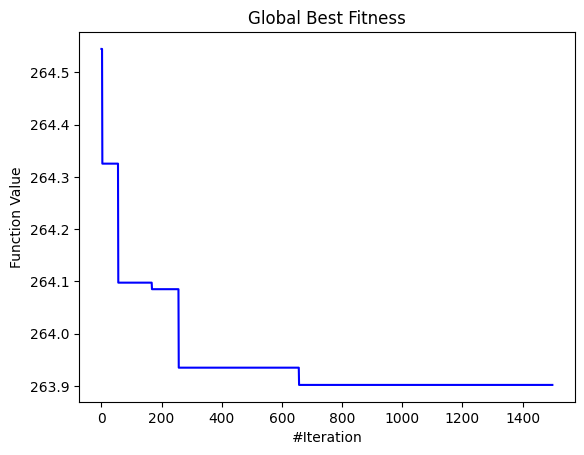
\includegraphics[width=.6\linewidth]{images/weight/400.png}
    \caption{Convergência do algoritmo genético com peso de penalização de 400.}%
    \label{fig:ga-weight-400}
\end{figure}

\begin{figure}
    \centering
    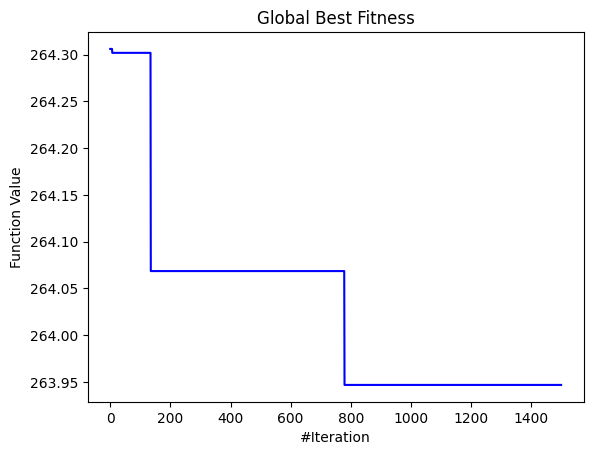
\includegraphics[width=.6\linewidth]{images/weight/800.png}
    \caption{Convergência do algoritmo genético com peso de penalização de 800.}%
    \label{fig:ga-weight-800}
\end{figure}

O algoritmo memético apresentou um desempenho semelhante, atingindo soluções próximas do ótimo em todas as execuções com pesos superiores a 100.
Além disso, sua convergência foi extremamente rápida, sendo que em algumas execuções uma única iteração foi suficiente para encontrar uma solução próxima do ótimo, com um valor aproximadamente uma unidade acima do ideal.

O gráfico do mínimo global poderia parecer sugerir uma estagnação, como mostrado na \autoref{fig:memetic-global}.
Entretanto, através do o gráfico do mínimo local mostrado em \autoref{fig:memetic-local}, é possível constatar que o algoritmo continuou a explorar o espaço de busca com expressiva variabilidade, até o limite de gerações estabelecido.

\begin{figure}
    \centering
    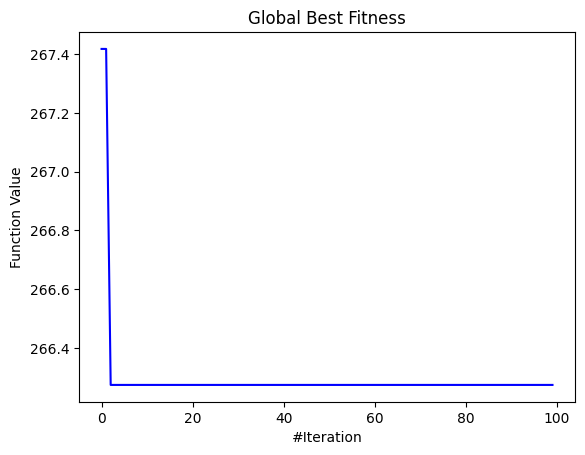
\includegraphics[width=.6\linewidth]{images/convergence/gdbf.png}
    \caption{Convergência do ótimo global para o algoritmo memético.}%
    \label{fig:memetic-global}
\end{figure}

\begin{figure}
    \centering
    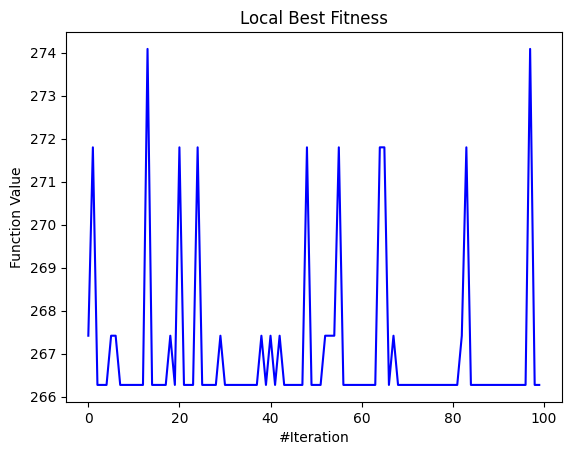
\includegraphics[width=.6\linewidth]{images/convergence/lbfc.png}
    \caption{Convergência do ótimo local para o algoritmo memético.}%
    \label{fig:memetic-local}
\end{figure}

Por outro lado, ao utilizar pesos de penalização mais baixos (50 ou inferiores), ambos os algoritmos começaram a gerar soluções inviáveis, como mostrado nas figuras~\ref{fig:non-viable-ga}, para o algoritmo genético, e~\ref{fig:non-viable-ma}, para o memético.

À medida que o peso diminuía, as soluções aparentavam melhorar em termos de qualidade, mas violavam cada vez mais as restrições, resultando em soluções que estruturalmente são impossíveis.
Comparativamente, o algoritmo memético se comportou de forma mais agressiva, gerando soluções inviáveis mais rapidamente que o algoritmo genético simples.

\begin{figure}
    \centering
    \begin{subfigure}{.5\textwidth}
        \centering
        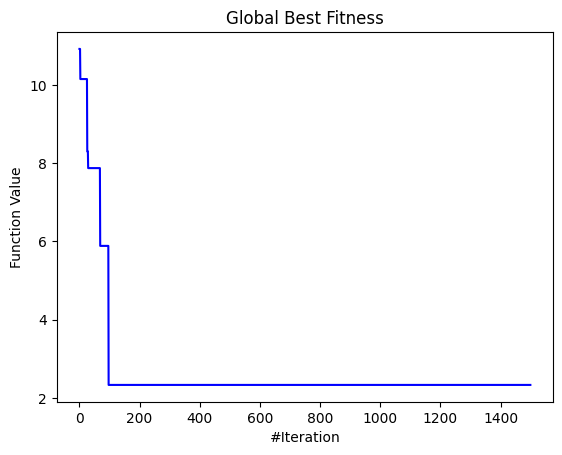
\includegraphics[width=1\linewidth]{images/non_viable/0/GA.png}
        \caption{Peso 0.}
    \end{subfigure}%
    \begin{subfigure}{.5\textwidth}
        \centering
        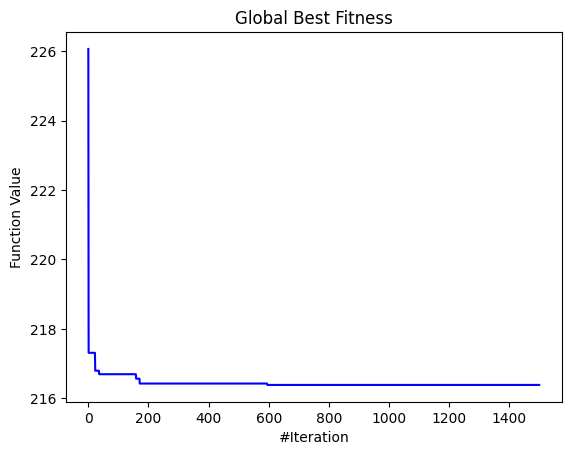
\includegraphics[width=1\linewidth]{images/non_viable/25/GA.png}
        \caption{Peso 25.}
    \end{subfigure}%
    \caption{Soluções inviáveis geradas pelo algoritmo genético.}%
    \label{fig:non-viable-ga}
\end{figure}

\begin{figure}
    \centering
    \begin{subfigure}{.5\textwidth}
        \centering
        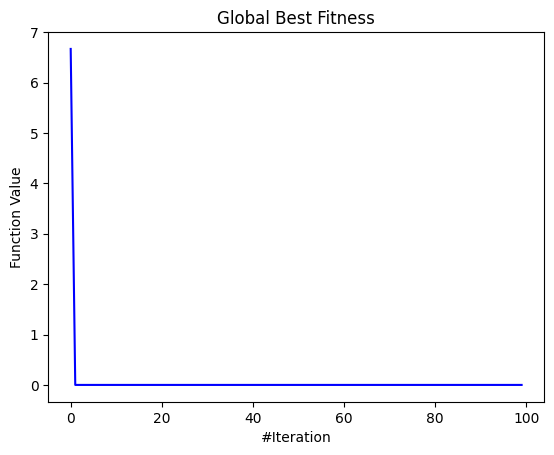
\includegraphics[width=1\linewidth]{images/non_viable/0/MA.png}
        \caption{Peso 0.}
    \end{subfigure}%
    \begin{subfigure}{.5\textwidth}
        \centering
        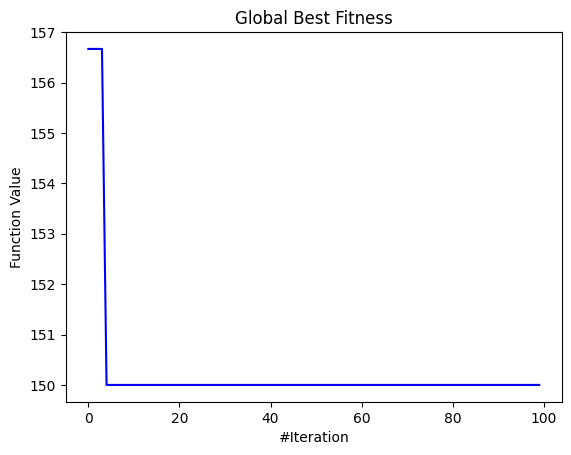
\includegraphics[width=1\linewidth]{images/non_viable/25/MA.png}
        \caption{Peso 25.}
    \end{subfigure}%
    \caption{Soluções inviáveis geradas pelo algoritmo memético.}%
    \label{fig:non-viable-ma}
\end{figure}
